\pagebreak
\section{Optimointimenetelmät}

Tässä luvussa esitellään muutamia menetelmiä, joilla kehittäjät ovat parantaneet virtuaalikoneidensa tuottaman konekoodin suorituskykyä. Optimointimenetelmiä on kehitetty moniin ongelma-alueisiin kuten kääntämiseen, muistinhallintaan ja kielen erityspiirteiden toteuttamiseen. Suuri osa menetelmistä hyödyntää virtuaalikoneen suoritusaikana keräämää profilointitietoa. Frankfurtin Goethe-yliopiston YouTube-kanavalta löytyy videoluentoja, joissa selitetään juurta jaksain englanniksi tässä luvussa esiteltyjä aiheita~\cite{goetheuni}.

\subsection{Piiloluokat}

JavaScriptin oliot käyttävät prototyyppiperintää. Tämä tarkoittaa, että oliolla on käytännössä aina jokin olio prototyyppinään, jolla on toinen olio prototyyppinään ja niin edelleen. Kun oliolta pyydetään jonkin \textit{ominaisuuden} (property) arvoa, etsitään sitä ensin itse oliosta. Jos ominaisuutta ei löydy, käydään olion prototyyppiketjua läpi, kunnes se löytyy tai kaikki prototyypit on käyty läpi, jolloin ominaisuuden arvoksi palautetaan \texttt{undefined}.

Ominaisuuden lisääminen tai muuttaminen päivittää oliota, ei koskaan sen prototyyppiä. Jos ominaisuutta ei ole oliossa, se lisätään siihen, vaikka kyseinen ominaisuus löytyisikin prototyyppiketjusta. Tällöin saman prototyypin omaavat oliot säilyttävän vanhan arvon ja vain muutettu olio käyttää uutta arvoa. Olion prototyyppiä pääsee kuitenkin muokkaamaan epästandardin \texttt{\_\_proto\_\_}-ominaisuuden kautta tai standardiin myöhemmin lisätyn \texttt{Object.getPrototypeOf(obj)}-funktion avulla.

Prototyyppiperintämallista johtuen ominaisuuksien arvot saattavat olla muistissa kaukana toisistaan ja niiden löytämiseen tarvitaan hidasta assosiatiivista hakurakennetta. Staattisissa luokkaperintään pohjautuvissa kielissä olioiden rakenne on helppo muuttaa prosessorille sopivampaan muotoon.

V8:n kehittäjät esittelivät ominaisuuden nimeltään \textit{piiloluokka} (hidden class)~\cite{v8design} ja sittemmin myös muita virtuaalikoneiden kehittäjiä on ottanut samanlaisen mallin käyttöön. Piiloluokat ovat \textit{muuttumattomia} (immutable) luokkia, joita virtuaalikone käyttää JavaScript-olioiden rakenteen kuvaamiseen. Piiloluokka on tavallaan siis olion tyyppi, vaikka JavaScriptissä olioilla ei ole varsinaisesti tyyppejä, paitsi kieleen sisäänrakennetut perustyypit, kuten \texttt{String} ja \texttt{Number}. Käyttämällä piiloluokkaa olion tyyppinä virtuaalikoneet voivat hyödyntää tehokkaita kääntämistekniikoita, joita käytetään yleisesti staattisesti tyypitetyissä kielissä.

Piiloluokat toimivat siten, että oliota luodessa ensimmäistä kertaa, virtuaalikone luo sille samalla piiloluokan. Aina kun oliota muutetaan lisäämällä siihen ominaisuus, luodaan sitä vastaamaan uusi piiloluokka tai käytetään olemassa olevaa piiloluokkaa. Piiloluokkia ei voi tehdä etukäteen, koska dynaamisuuden takia on vaikea tietää ennalta millainen olio tulee rakenteeltaan olemaan. 

Kuvassa~\ref{fig:hiddenclass} näkyy, miten V8 luo piiloluokkia luodessaan Piste-olion ensimmäisen kerran. Jokainen kaavion askel vastaa yhden koodirivin suorittamista. Kun konstruktorifunktiota kutsutaan, luodaan tyhjä olio, johon viitataan avainsanalla \texttt{this}. Virtuaalikone kuvaa sitä tyhjällä piiloluokalla \texttt{C0}. Luokkaa \texttt{C0} käytetään kuvaamaan kaikkia tyhjiä olioita, joilla on sama prototyyppi, joka on oletuksena kieleen sisäänrakennetun \texttt{Object}-olion ilmentymä. Konstruktorissa olioon liitetään ominaisuus \texttt{x}, jolloin virtuaalikone luo uuden piiloluokan \texttt{C1} ja lopulta \texttt{y}:n lisäyksen jälkeen \texttt{C2}:n. Piiloluokkiin tallennetaan myös tieto mihin luokkaan pitää siirtyä tietyn ominaisuuden lisäämisen jälkeen sekä viittaus olion prototyyppiin.

\begin{figure}[ht]
    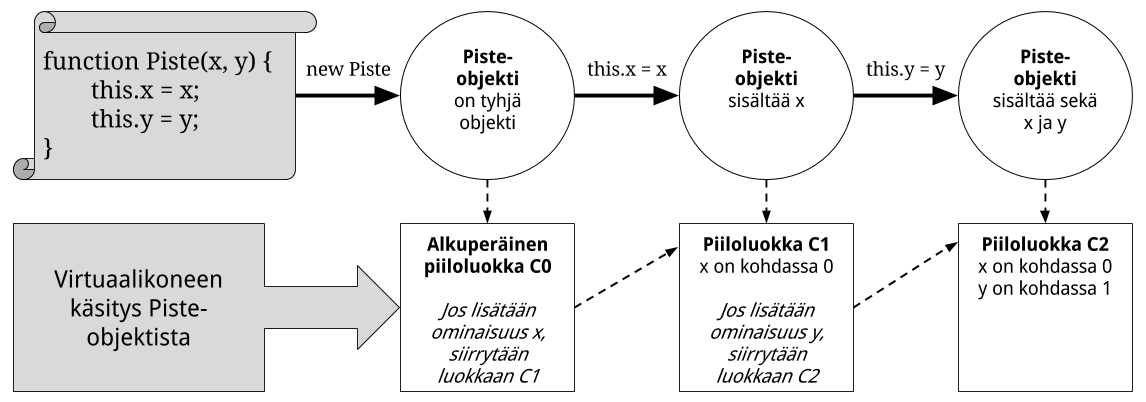
\includegraphics[width=\textwidth]{hidden-classes}
    \caption{Esimerkki piiloluokkien toimintaperiaatteesta.}
     \centering
     \label{fig:hiddenclass}
\end{figure}

Piiloluokkia ei tarvitse luoda uudestaan joka kerta, kun halutaan luoda uusi Piste-olio. Riittää, että seurataan niihin sisällytettyjä tietoja siirtymistä. Kun uusi Piste-olio luodaan, päädytään lopulta samaan piiloluokkaan \texttt{C2}. Kaikki Piste-oliot ovat siis virtuaalikoneen näkökulmasta samantyyppisiä.

Kun Piste-oliolta pyydetään esimerkiksi ominaisuuden \texttt{x} arvoa, virtuaalikone tietää, että olio on luokan \texttt{C2} ''tyyppinen'' ja arvo löytyy yhdellä konekäskyllä olion muistipaikasta siirtymällä 0 ilman, että täytyy tehdä hidasta hakua assosiatiivisesta hakurakenteesta. Virtuaalikone voi siis generoida tehokkaampaa konekoodia ja muistiviittaukset nopeutuvat huomattavasti.

Syy, miksi luodaan useita piiloluokkia yhden olion luonnin yhteydessä on, että niihin lisätyt siirtymätiedot mahdollistavat erilaisten olioiden luomisen käyttäen hyväksi jo luotuja piiloluokkia. Esimerkiksi \texttt{Ympyrä}-olio voi sisältää ominaisuudet \texttt{x}, \texttt{y} ja \texttt{r}, jolloin sen luomisessa käytetään piiloluokkia \texttt{C0}, \texttt{C1}, \texttt{C2} ja luodaan uusi \texttt{C3}. Vaihtoehtoisesti voimme luoda kolmiulotteisen Pisteen, jolla on tasokoordinaattien lisäksi \texttt{z}-ominaisuus. Tällöin piiloluokka \texttt{C2} sisältää tiedon siirtymästä molemmissa, ympyrän ja kolmiulotteisen pisteen, tapauksissa.

Wonsun Ahn kumppaneineen on tutkinut piiloluokkien hyötyjä ja haittoja todellisissa verkkosovelluksissa~\cite{Ahn2014}. Tutkimuksessa on löytynyt muutamia heikkouksia, jotka vähentävät piiloluokkien hyötyjä todellisissa sovelluksissa ja heikkouksiin ehdotetaan parannuksia. Siinä myös moititaan kehittäjien vahvaa oletusta ohjelmien staattisesta käytöksestä. Tutkimuksessa havaittiin, miten dynaamisuutta paljon hyödyntävä ohjelma voi helposti luoda paljon piiloluokkia turhaan esimerkiksi alustamalla ominaisuuksia eri järjestyksessä eri kerroilla tai ehdollisesti. Jos piiloluokkia on paljon se haittaa optimointien, kuten sisällytetyn välimuistin, toimivuutta.

\subsection{Sisällytetty välimuisti}

\textit{Hakupaikaksi} (access site) kutsutaan kohtaa koodissa, jossa viitataan olion ominaisuuteen. Koska muuttujilla ei ole tyyppiä, virtuaalikone ei voi tietää ennalta löytyykö edes kyseistä ominaisuutta. Yleinen olettamus on, että samalla hakupaikalla oliot ovat usein samantyyppisiä. Tämän takia esimerkiksi V8:ssa on alettu käyttää \textit{sisällytettyä välimuistia} (inline cache)~\cite[s.~498]{Ahn2014}. Nimi tulee siitä, että välimuisti on osa generoitua konekoodia. Sen tehtävä on tarkistaa vastaan tulevien arvojen tyyppi ja tallentaa profilointitietoa optimoivaa kääntäjää varten. Sillä ei siis ole suoraan tekemistä prosessorin välimuistin kanssa.

Tarkastellaan seuraavaa pseudokoodia:
\begin{lstlisting}
function getX(obj) { return obj.x; }
var p = new Piste(1, 2)
for (var i = 0; i < 100000; i++) getX(p);
\end{lstlisting}
Keräämällä tietoa suoritusaikana virtuaalikone voi päätellä, että hakupaikassa \texttt{obj.x} on \texttt{obj}-muuttujan arvona usein Piste-olio. Virtuaalikone voi muokata konekoodia ja lisätä tarkistuksen: ''Onko \texttt{obj}:n piiloluokka \texttt{C2}?'' Jos oliolla on tämä piiloluokka, arvon lukemisen voi suorittaa yhdellä konekäskyllä, sillä ominaisuuden siirtymä muistissa on tunnettu piiloluokan rakenteesta. Sitä voisi kuvata esimerkiksi pseudokoodilla:
\begin{lstlisting}
if (haePiiloluokka(obj) == 'C2') return obj[C2_X_OFFSET];
else return teeHidasHaku(obj, 'x');
\end{lstlisting}

V8:ssa on kolmen tyyppisiä sisällytettyjä välimuisteja: \textit{lataukselle} (load), \textit{talletukselle} (store) ja \textit{kutsumiselle} (call). Lataaminen tarkoittaa olion ominaisuuden hakemista ja talletus sen päivittämistä. Kutsuminen tarkoittaa olioon liitetyn funktion kutsumista ja se on samankaltainen lataamisen kanssa, sillä ensin pitää ladata funktio, joka on JavaScriptissä viittaus funktio-olioon.

Jos olion tyyppiä ei löydy sisällytetystä välimuistista, V8 voi lisätä tarkistuksen sisällytettyyn välimuistiin. Esimerkiksi, jos ohjelma alkaa kutsua \texttt{getX}-funktiota ympyräolioilla, V8 voi lisätä sisällytettyyn välimuistiin tarkistuksen: ''Onko \texttt{obj}:n piiloluokka \texttt{C3}?''. Tällöin arvon voi ladata taas nopeasti tunnetusta siirtymästä pseudokoodilla:
\begin{lstlisting}
if (haePiiloluokka(obj) == 'C2') return obj[C2_X_OFFSET];
else if (haePiiloluokka(obj) == 'C3') return obj[C3_X_OFFSET];
else return teeHidasHaku(obj, 'x');
\end{lstlisting}

Ylimääräiset tarkistukset tekevät suorituksesta tietenkin hitaampaa. Tutkimuksen mukaan haku välimuistin avulla voi olla parhaimmillaan monta kertaluokkaa nopeampaa kuin ilman välimuistia~\cite[s.~498]{Ahn2014}, koska silloin ei tarvitse tehdä hidasta hakua ominaisuuden nimellä.

\subsection{Aktivaatiotietueiden manipulointi}

Normaalisti JIT-kääntäjät ottavat optimoidun funktion käyttöön vasta seuraavalla funktion kutsukerralla. Tämä lähestymistapa toimii hyvin monissa tapauksissa, mutta ei silloin kun funktio sisältää esimerkiksi monesti suoritettavan toistorakenteen. Jos funktiota kutsutaan vain kerran, optimoitua koodia ei koskaan saada käyttöön.

Tätä varten on kehitetty menetelmä, jonka englanninkielinen nimi on ''on-stack replacement''~\cite{osr}. Suomeksi menetelmää voi kutsua aktivaatiotietueiden manipuloinniksi. Kuvassa~\ref{fig:osr} näkyy kuinka menetelmää voi käyttää funktion \texttt{f} optimointiin.

\begin{figure}[ht]
    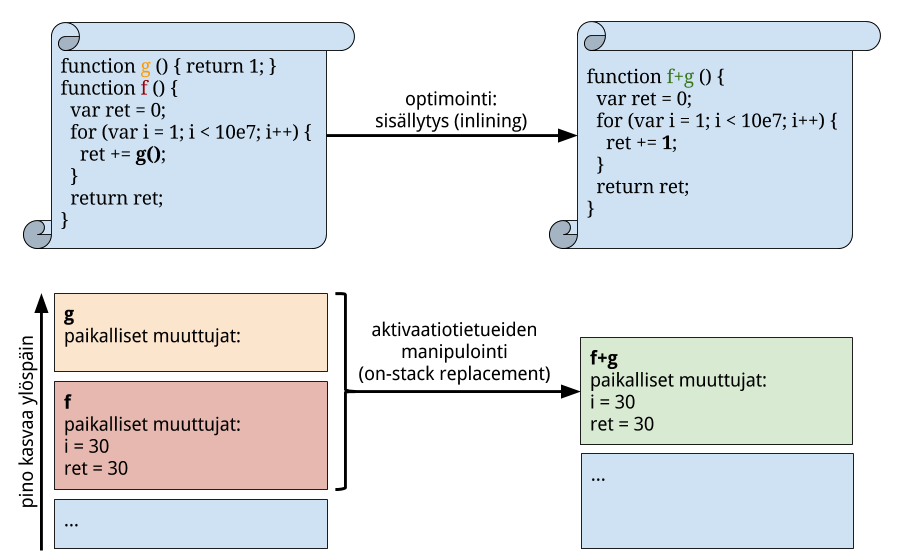
\includegraphics[width=\textwidth]{on-stack-replacement}
    \caption{Esimerkki aktivaatiotietueiden manipuloinnista~\cite{osrpic}.}
     \centering
     \label{fig:osr}
\end{figure}

Kun virtuaalikone alkaa ensimmäistä kertaa suorittaa funktiota \texttt{f}, sitä ei ole vielä optimoitu. Virtuaalikone kerää JIT-kääntämistä varten tietoa suorituksen kulusta aika ajoittain ja huomaa, että funktion suoritus vie paljon aikaa ja funktio pitäisi optimoida. Virtuaalikoneen optimointiheuristiikka päättää sisällyttää funktion \texttt{g} funktion \texttt{f} sisään eliminoiden turhan funktiokutsun. Esimerkissä tämä tapahtuu 30. toiston kohdalla.

Kun optimoitu funktio \texttt{f+g} on käännetty, suoritus pitää siirtää funktiosta \texttt{f} uuteen funktioon \texttt{f+g}. Koska funktion \texttt{f} suoritus on kesken, täytyy manipuloida funktion \texttt{f} aktivaatiotietuetta pinossa, siten että se sisältää myös funktion \texttt{g} mahdolliset paikalliset muuttujat. Tässä esimerkissä sellaisia ei ole, mutta todellisessa tapauksessa virtuaalikoneen täytyy luoda kuvaus molemmista aktivaatiotietueista yhdistetyn funktion \texttt{f+g} aktivaatiotietueeksi.

Aktivaatiotietueiden manipuloinnin täytyy toimia myös toiseen suuntaan, eli jos koodissa tulee vastaan tapaus, jota optimointi ei ottanut huomioon, täytyy optimointi pystyä peruuttamaan, jolloin aktivaatiotietue pitää pilkkoa osiin taas. Menetelmään liittyy paljon teknisiä yksityiskohtia, kuten miten pysäyttää funktion suoritus ja miten manipuloida aktivaatiotietueita oikein. Tästä huolimatta suurin osa JavaScript-virtuaalikoneista on ottanut menetelmän käyttöön. Toteutuksessa auttaa, jos virtuaalikone hallitsee kaiken konekoodin generoimista, koska silloin se voi esimerkiksi rajoittaa funktiokutsujen konventioita konekoodissa ja vähentää mahdollisten ongelmatilanteiden lukumäärää.

\subsection{Roskienkeruu}

JavaScript-virtuaalikoneiden \textit{roskienkeruu} (garbage collection) on perinteisesti toiminut melko yksinkertaisella algoritmilla nimeltään \textit{merkitse ja pyyhkäise} (mark-and-sweep). Algoritmi perustuu nimensä mukaisesti kahteen vaiheeseen. Ensimmäinen on merkitsemisvaihe, jossa käydään läpi kaikki ohjelman viittaamat oliot ja merkitään ne. Sitten seuraa pyyhkäisyvaihe, jossa koko muisti käydään läpi ja vapautetaan kaikki oliot, jotka eivät ole merkittyjä ja samalla poistetaan merkit seuraavaa suoritusta varten.

Ohjelman suoritus ei voi jatkua roskienkeruun aikana, koska ohjelma voi käyttää muistia milloin vain, ja koko muistialueen käsitteleminen on hidasta. Tämä on suuri ongelma varsinkin animaatioiden ja interaktiivisten sovellusten tapauksessa, sillä pitkä roskienkeruutauko haittaa käytettävyyttä ja saa sovelluksen tuntumaan hitaalta, vaikka muu suoritus olisikin todella nopeaa.

Ongelman ratkaisemiseksi on kehitetty monenlaisia heuristiikkoja ja optimointeja. Automaattisesta muistinhallinnasta riittää materiaalia useampaankin tutkielmaan~\cite{gcbib}. Tässä on lista joitain esimerkkejä menetelmistä, joilla roskienkeruuta on parannettu:

% TODO: Viittaus periaatteeseen, eikä toteutukseen.

\begin{itemize}
\item \textit{sukupolvittainen roskienkeruu} (generational garbage collection)~\cite{v8design}
\item \textit{inkrementaalinen roskienkeruu} (incremental garbage collection)~\cite{incrementalgc}
\item roskienkeruu ''luppoaikana'' eli roskienkeruun aikataulutus~\cite{freegc}
\item muistin jakaminen eri osiin, joiden keruuta voi rinnakkaistaa~\cite{ie10}.
\end{itemize}